
%
%=============================================================================
%
%
% Slide
%
\section{Grapical User Interface (GUI)}
%
% Slide
%
\begin{frame}[fragile]\frametitle{GUIs in MATLAB}
\begin{itemize}
\item Das Graphical User Interface(GUI) erm\"oglicht das Steuern von Programmen
  mit Hilfe der grafischen Oberfl\"ache. 
\item Programme können von Usern ohne MATLAB-Kenntnisse genutzt werden. 
\item Hilfreich selbst für den Implementierer von numerischen Algorithmen.
\item Steuerung der GUIs durch Grafik-Objekte der Typen
\begin{itemize}
\item \mcode{uimenu}
\item \mcode{uicontextmenu} 
\item \mcode{uicontrol}
\item \mcode{uipanel}
\end{itemize}
(Gleiche Hierachie-Ebene wie \mcode{axes}-Objekte)
\item Grafische Oberfl\"ache zur Erstellung von GUIs:
\begin{matlabin}
guide
\end{matlabin}
 
\end{itemize}
\end{frame}
%
% Slide
%
\begin{frame}[fragile]\frametitle{Vordefinierte GUIs f\"ur Dialogboxen}
\begin{itemize}
\item { \mcode{helpdlg}}: Hilfebox
\item { \mcode{msgbox}}: Eine beliebige Nachricht
\item { \mcode{warndlg}}: Anzeige einer Warnung
\item { \mcode{inputdlg}}: Abfragen einer Gr\"o{\ss}e
\item { \mcode{questdlg}}: Frage
\end{itemize}
\alert{Beispiel:}
\begin{matlabin}
h1 = warndlg('NameFenster','Nachricht')
h2 = errordlg('NameFenster','Nachricht')
ans = questdlg('NameFenster','Nachricht')
ant = inputdlg({'Frage 1','Frage 2','Frage3'},...
  'NameFenster',[1 2 3], {'defAnt1','defAnt2','defAnt3'})
\end{matlabin}
\end{frame}
%
% Slide
%
\begin{frame}[fragile]\frametitle{Grafik-Objekte und GUIs}
\begin{itemize}
\item \alert{ uicontrol}:
Interaktive grafische Objekte, die Aktionen steuern oder bestimmte Optionen setzen.

\item \alert{ uimenu}:
Benutzerdefinierte Men\"uf\"uhrung in einer \mcode{figure} (wird nicht behandelt).

\item \alert{ uicontextmenu}:
Ein Pop-up Men\"u, das erscheint, wenn der Benutzer mit der rechten Maustaste
ein grafisches Objekt anklickt (wird nicht behandelt).
\item \alert{uipanel}:
  Container-Objekt zum Gruppieren von anderen Elementen.
\end{itemize}
\end{frame}
%
% Slide
%
\begin{frame}[fragile]\frametitle{Arten von UiControls}
\centering
\begin{tabular}{ll}
\mcode{'checkbox'} & Wahl von Zust\"anden an/aus \\
\mcode{'edit'}     & Editierbare Texteingabe\\
\mcode{'popup'}    & Auswahl aus Liste bei Anklicken\\ 
\mcode{'listbox'}  & Auswahl aus einer skrollbaren Liste \\
\mcode{'pushbutton'} & Starten eines Events \\
\mcode{'radio'}    & Auswahl einer Option \\
\mcode{'toggle'}  & Wahl des Zustandes: an/aus  \\
\mcode{'slider'}   & Auswahl aus Wertebereich\\
\mcode{'text'}     & Anzeige von Text in einer Box\\
\end{tabular}

\end{frame}
%
% Slide
%
\begin{frame}[fragile]\frametitle{Eigenschaften von UiControls}
\begin{tabular}{lp{0.85\linewidth}}
Style & Art des UiControls \\
\hline
CallBack & Durch Anklicken des Users auszuf\"uhrende Aktion\\
Position & Lage des Uicontrol-Objekts in der \mcode{figure}\newline
          {\scriptsize Eingabe: [links unten Breite H\"ohe]} \newline
          {\scriptsize Einheiten werden durch die \mcode{Units}-Eigenschaft gesteuert.}\\
String   & Textdarstellung. Bei mehreren Optionen durch Eingabe \newline
          {\scriptsize \mcode{string=\{'opt1';'opt2'\}} oder
            \mcode{string='opt1\|opt2'}}\\
Units    & Einheit zur Bestimmung der Lages des UiControls,\newline
          {\scriptsize Werte: \mcode{pixels} (Default), \mcode{centimeters},
          \mcode{normalized} (Werte in $[0,1]$)}\\
Tag      & String zum Auffinden des Objekts durch \mcode{findobj}
\end{tabular}
\end{frame}
%
% Slide
%
\begin{frame}[fragile]\frametitle{Erzeugen von UiControls}
UiControl-Objekte k\"onnen durch \alert{ \mcode{uicontrol}} erzeugt
werden. Aufruf: 
\begin{matlabin}
handle = uicontrol('<eig1>',<wert1>,.., '<eign>',<wertn>)
\end{matlabin}
\alert{Beispiel:}
\begin{matlabin}
u = uicontrol('style','listbox',...
'string','Option1|Option2|Option3',...
'units','centimeters','position',[0 0 3 3])
\end{matlabin} 
\end{frame}

%
% Slide
%
\begin{frame}[fragile]\frametitle{CallBack}
\begin{itemize}
\item Sobald ein GUI-Objekt aktiviert wird, f\"uhrt es MATLAB Code aus. Dies
  wird {\it CallBack} genannt.
\item {\it CallBack} ist eine Eigenschaft von UiControl.
\item Ein GUI-Objekt wird in der Regel durch einen Mausklick oder \"ahnliches
  aktiviert. 
\item CallBack kann eine Funktion oder ein String, der durch \mcode{eval}
  ausf\"uhrbar ist, sein. 
\item Syntax der Callback-Funktion (durch \mcode{guide} erstellt)

\end{itemize}
\end{frame}

%
% Slide
%
\begin{frame}[fragile]\frametitle{CallBack - Syntaxvarianten}
\begin{itemize}
 \item \mcode{function myfile} \\
\mcode{set(h, 'CallBack', 'myfile')}\\
\item \mcode{function myfile(obj, event)} \\
 \mcode{set(h, 'CallBack', @myfile)}\\
\item \mcode{function myfile(obj, event, arg1, arg2)}\\ 
\mcode{set(h, 'CallBack', \{'myfile', 5, 6\})}\\
\item \mcode{function myfile(obj, event, arg1, arg2)}\\ 
\mcode{set(h, 'CallBack', \{@myfile, 5, 6\})}\\
 \item GUIDE
   \begin{matlabin}
function varargout = <objectTag>_Callback(h,ev_data,handles, varargin)}}     
   \end{matlabin}
\begin{itemize}
\item \mcode{objectTag}: ist der Name, der im Tag des Objects gespeichert wird.
\item \mcode{h}: ist der Handle des Objekts, dass die CallBack-Funktion
  aufruft. 
\item \mcode{ev_data}: event-data (normalerweise unnötig).
\item \mcode{handles}: Struktur aller Objekte in der GUI
\item \mcode{varargin}: ist eine  Liste von Argumenten, die an die Funktion
  \"ubergeben wird.  
\end{itemize}
\end{itemize} 
\end{frame}

% 
% Slide
% 
\begin{frame}[fragile]\frametitle{Hinweise}
\begin{itemize}
\item Callback-Funktionen werden immer im Haupt-Workspace
  gestartet. 
\item Mit Hilfe der \mcode{figure}-Eigenschaft \mcode{UserData} k\"onnen Daten an
  das \mcode{figure}-Objekt geh\"angt werden.
\item Der User kann grafische Objekte per Hand schlie{\ss}en. Dies kann zu
  falschen Aufrufen f\"uhren.
\item Man achte darauf, dass man die richtigen Objekte anspricht. Tipp:
  Eigenschaft \mcode{Tag}. 
\item \mcode{hold (<axes_handle>)}: Verhindern, dass Axen-Einstellungen durch nachfolgende plot-Befehle überschrieben werden.
\end{itemize}
\end{frame}
% 
% Slide
%
\begin{frame}[fragile]\frametitle{Beispiel einer GUI}
\begin{center}
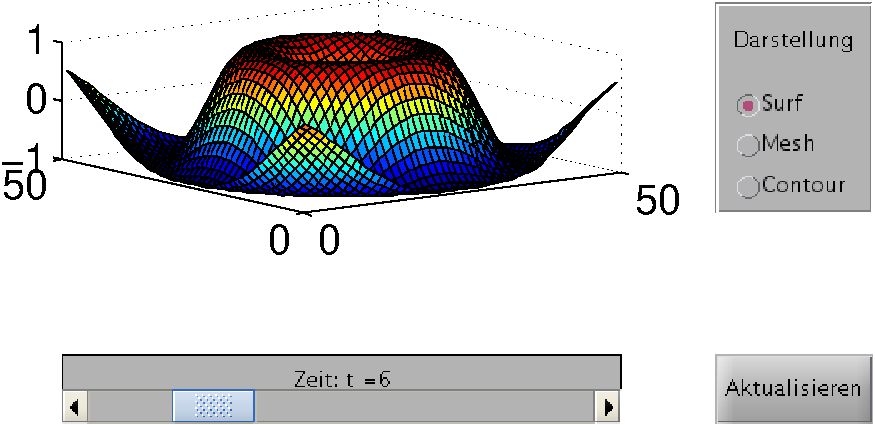
\includegraphics[width=0.9\textwidth]{./figures/gui}
\end{center}
\end{frame}
% 
% Slide
%
\begin{frame}[fragile]\frametitle{bild\_funktion.m}
\begin{matlabin}
function han = bild_funktion()
x = linspace(-1,1,50);
y = linspace(-1,1,50);
t = 0:1:30;
A = erzDaten(x,y,t);
han = erzGUI(A);
end
%------------------- Grafische Oberflaeche erzeugen
function han = erzGUI(A);
delete(findobj('tag','figGUI'));
fig = figure('name','Beispiel GUI','UserData',A,'tag','figGUI');
han.pushbutton = uicontrol(fig,'Parent',fig,'Style',...
  'pushbutton','units','normalized','position',...
  [0.8 0.2 0.15 0.15],'String','Aktualisieren',...
  'Callback','darstGrafik');
han.grafikachse = axes('Position',[0.1 0.5 0.6 0.3],'tag','axesGUI');
han.grafik = surf(A(:,:,1));
\end{matlabin}
\end{frame}
% 
% Slide
%
\begin{frame}[fragile]\frametitle{bild\_funktion.m}
\begin{matlabin}
han.frame1 = uicontrol(fig,'style','frame', 'units',...
  'normalized','position',[0.1 0.2 0.6 0.1]);
han.slider = uicontrol(fig,'style','slider','sliderstep',...
  [0.2 0.2],'min',0,'max',30, 'units','normalized',...
  'position', [0.1 0.2 0.6 0.05],'tag','slider',...
  'Callback','darstGrafik');
han.text1 = uicontrol(fig,'style','text', 'tag',...
  'text1','units','normalized','position', ...
  [0.3 0.25 0.1 0.03],'String','Zeit t = 0');
han.frame2=uibuttongroup('units','normalized','tag','radio',...
  'position',[0.8 0.5 0.15 0.3]);
han.text2=uicontrol(fig,'style','text','parent',han.frame2,...
  'units','normalized','position', [0.1 0.6 0.8 0.3],...
  'String','Darstellung');
\end{matlabin}
\end{frame}
% 
% Slide
%
\begin{frame}[fragile]\frametitle{bild\_funktion.m}
\begin{matlabin}
han.radio1=uicontrol(fig,'style','radio','parent',han.frame2,...
  'tag','r1', 'units','normalized',...
  'position', [0.1 0.45 0.8 0.15],'String','Surf');
han.radio2=uicontrol(fig,'style','radio','parent',han.frame2,...
  'tag','r2','units','normalized',...
  'position', [0.1 0.25 0.8 0.15],'String','Mesh');
han.radio3=uicontrol(fig,'style','radio','parent',han.frame2,...
  'tag','r3','units','normalized',...
  'position', [0.1 0.05 0.8 0.15],'String','Contour');
end
function A = erzDaten(x,y,t)
[X,Y,T] = meshgrid(x,y,t);
A = cos(pi*T.^0.5.*exp(-X.^2-Y.^2));
end
\end{matlabin}
\end{frame}
% 
% Slide
%
\begin{frame}[fragile]\frametitle{darstGrafik.m}
\matinput{darstGrafik.m}
\end{frame}
